\documentclass{beamer}
\usefonttheme[onlylarge]{structuresmallcapsserif}
\usefonttheme[onlysmall]{structurebold}
\usetheme{Warsaw}
\setbeamercovered{transparent}

\usepackage{fancybox,color,tcolorbox}
\usepackage{verbatim}
\usepackage[english,spanish,activeacute]{babel}
%\usepackage[latin1]{inputenc}
\usepackage{inputenc}
\usepackage{latexsym}
\usepackage{amsmath}
\usepackage{graphicx} % Allows including images
\usepackage{booktabs}
\usepackage{amssymb}
\usepackage{multimedia}
\usepackage{pifont,pgfcore}
\usepackage{tcolorbox}
\usepackage{animate}
\usepackage{ucs}

\title[Carlos Daniel Largacha Leal C-112]{Proyecto de Programación I \\ Moogle!.}
\author[Proyecto I Moogle!]{Carlos Daniel Largacha Leal \\ C-112}
\date{}

\begin{document}
\begin{frame}
	 \titlepage
	\begin{center}
		\colorbox{black}{\textbf{\begin{large}\textcolor{white}{Universidad de la Habana}\end{large}}}\\\ \\
		\scriptsize \textbf{\textcolor{blue}{Facultad Matemática y Computación}}\\
	\end{center}
\end{frame}

\begin{frame}
		\frametitle{Temas a tratar} 
	\begin{itemize}
		\item  Ejecución del Moogle!
		\item  ¿Qué hace el programa?
		\item  Funcionamineto del Programa
		\item  Tf-idf
		\item  Distancia Levenshtein
	\end{itemize} 
\end{frame}

\begin{frame}
	\frametitle{Ejecución del Moogle!} 
	\begin{itemize}
    \item  Copiar a la carpeta “Content” los documentos
    \item  Asegurarse de que los documentos sean de extensión “.txt”
    \item  Ejecutar el programa
	\end{itemize} 
\end{frame}

\begin{frame}
	\frametitle{¿Qué hace el programa?} 
	\begin{figure}
		
\includegraphics[width=10cm]{moogle.png}
		\label{Lupita}
		\caption{Interfaz gráfica del Moogle!}
    \end{figure}
\end{frame}	

\begin{frame}
	\frametitle{Funcionamineto del Programa} 
	
	\begin{center}
	\textbf{\begin{large}\textcolor{blue}{Clases del Programa}\end{large}}\\
    \end{center}
    
	\begin{itemize}
		\item  Moogle: clase principal del proyecto.
		\item  Ordenar: clase encargada de ordenar los resultados de búsqueda.
		\item  Searchitem: información acerca de los documentos que responden a la búsqueda.
		\item  Searchresult: representa el resultado de la búsqueda
		\item  Suggestion: provee una sugerencia a partir de la consulta del usuario
		\item  TF$-$IDF: convierte el conjunto de documentos en una matriz de vectores
		\item  Utilidades: multiplica una lista de números decimales (donde se encuentra el tf$-$idf 
		de la consulta) y se multiplica por una lista de matrices.   
	\end{itemize}
\end{frame}	

\begin{frame}
	\frametitle{tf-idf} 
	     El tf-idf es el producto de dos medidas:\\.\\
         $tf-idf(t,d,D) = tf(t,d) * idf(t,D)$\\ .\\
         tf(t,d) representa la frecuencia de una palabra t en un documento d, es decir la cantidad de veces que una palabra se repite en un documento.\\.\\
         $idf(D,t) = log\dfrac{D}{d(t)}$
\end{frame}

\begin{frame}
	\frametitle{Distancia Levenshtein} 
		\begin{figure}
		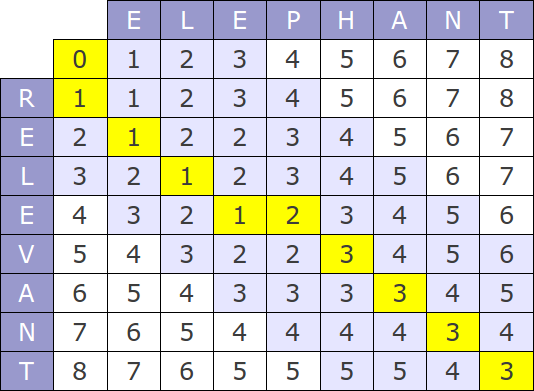
\includegraphics[width=7cm]{Levenshtein.png}
		\label{Leve}
		\caption{Distancia de dos palabras empleando el algoritmo Levenshtein}
	\end{figure}
\end{frame}	
\end{document}